\documentclass[varwidth=true]{standalone}
\usepackage{tikz}
\begin{document}
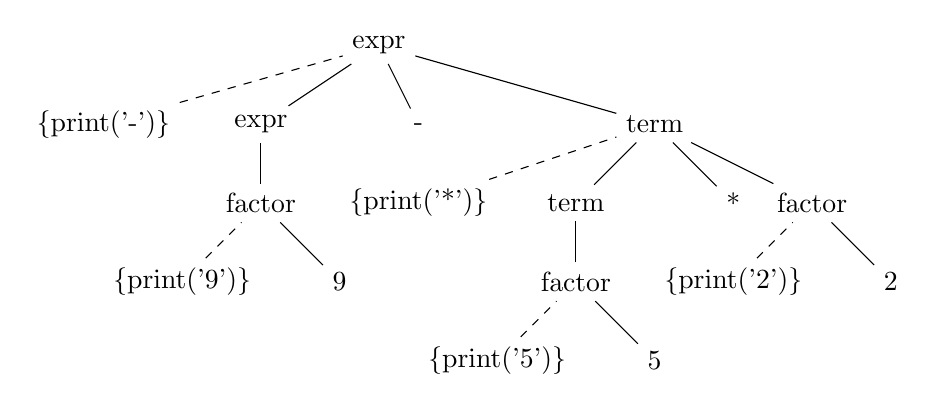
\begin{tikzpicture}
  \node (p5) at (4, 0) {\{print('5')\}};
  \node (5) at (6, 0) {5};

  \node (p9) at (0, 1) {\{print('9')\}};
  \node (9) at (2, 1) {9};
  \node (f5) at (5, 1) {factor};
  \node (p2) at (7, 1) {\{print('2')\}};
  \node (2) at (9, 1) {2};

  \draw[dashed] (p5) -- (f5);
  \draw (5) -- (f5);

  \node (f9) at (1, 2) {factor};
  \node (p*) at (3, 2) {\{print('*')\}};
  \node (t5) at (5, 2) {term};
  \node (*) at (7, 2) {*};
  \node (f2) at (8, 2) {factor};

  \draw[dashed] (p9) -- (f9);
  \draw (9) -- (f9);
  \draw (f5) -- (t5);
  \draw[dashed] (p2) -- (f2);
  \draw (2) -- (f2);

  \node (p-) at (-1, 3) {\{print('-')\}};
  \node (e9) at (1, 3) {expr};
  \node (-) at (3, 3) {-};
  \node (t*) at (6, 3) {term};

  \draw (f9) -- (e9);
  \draw[dashed] (p*) -- (t*);
  \draw (t5) -- (t*);
  \draw (*) -- (t*);
  \draw (f2) -- (t*);

  \node (e) at (2.5, 4) {expr};

  \draw[dashed] (p-) -- (e);
  \draw (e9) -- (e);
  \draw (-) -- (e);
  \draw (t*) -- (e);
\end{tikzpicture}
\end{document}
